\documentclass{report}
\usepackage{amsmath}
\usepackage{libertine}
\usepackage{tikz}
\usetikzlibrary{intersections}
\usetikzlibrary{through}
\usetikzlibrary{angles}
\usetikzlibrary{calc}
\usetikzlibrary{quotes}

\begin{document}

$
r_{\!_{11}} = -r\cos(\theta -\alpha) + \sqrt{\strut R_1^2 - r^2\sin^2(\theta - \alpha)}
$
\\
\\
$
r_{\!_{12}} = R_1 \cos \alpha - r\cos(\theta - \alpha)  + \\ ~ \qquad \sqrt{\strut [R_1 \cos \alpha - r\cos(\theta-\alpha) ]^2 - r^2\sin^2 \theta - [R_1 - r\cos \theta]^2 + R_2^2}
$
\\
\begin{align*}
\rho(r,\theta) &=  \int_{-\alpha_2}^{\alpha_1} f_{\alpha}(\alpha) \int_{r_{\!_{11}}}^{\infty} f_l(l)dl d\alpha +  \int^{2\pi-\alpha_2}_{\alpha_1} f_{\alpha}(\alpha) \int_{r_{\!_{12}}}^{\infty} f_l(l)dl d\alpha  \\
&=\int_{-\alpha_2}^{\alpha_1} \frac{1}{2\pi} e^{-\lambda \pi r_{\!_{11}}^2} d\alpha +  \int^{2\pi-\alpha_2}_{\alpha_1} \frac{1}{2\pi} e^{-\lambda \pi r_{\!_{12}}^2} d\alpha
\end{align*}
\\
\begin{tikzpicture}
	\draw (-1.5,0) -- (1.5,0);
	\draw (0,-1.5) -- (0,1.5);
	\draw (0,0) circle [radius=1cm];
\end{tikzpicture}
\\
\begin{tikzpicture}[scale=0.05]
	\coordinate [label=left:{\small $BS$}] (A) at (0,0);
	\fill [red,opacity=.5] (A) circle (50pt);
	
	\coordinate [label=right:{\small $U$}] (B) at (150,0);
	\fill [green,opacity=.5] (B) circle (50pt);
	
	\coordinate [label=above:{\small $R$}] (C) at (125,50);
	\fill [blue,opacity=.5] (C) circle (50pt);

	\draw (A) -- node[below=2pt] {\small $R_0$} (B) -- node[right=2pt] {\small $r_2$} (C)
	-- node[above=2pt] {\small $r_1$} cycle;
	
\end{tikzpicture}
\\
\begin{align*}
	\text{policy:}& \{P^b r_1^{-\alpha} < P_b R_0^{-\alpha}, P_rr_2^{-\alpha} > P_bR_0^{-\alpha}\} 
	\\
	& \{ r_1 < R_0, r_2 < R_2 \}
\end{align*}
where $ R_2 = cR_0, c = \big(\frac{P_a}{P_b}\big)^{\frac{1}{\alpha}} < 1 $
	\\
\centering{
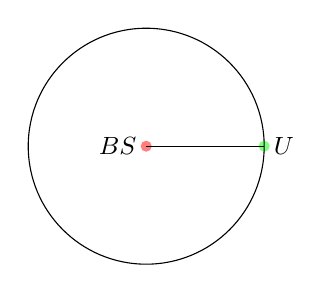
\begin{tikzpicture}[scale=0.01]
	\coordinate [label=left:{\small $BS$}] (A) at (0,0);
	\coordinate [label=right:{\small $U$}] (B) at (150,0);
	\fill [red,opacity=.5] (A) circle (200pt);
	\fill [green,opacity=.5] (B) circle (200pt);

	\draw (A) -- (B);
	\node (D) [name path=D,draw,circle through=(B)] at (A) {};
\end{tikzpicture}
	}
	\\
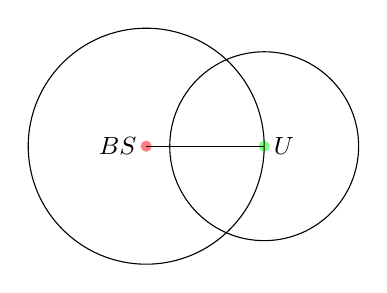
\begin{tikzpicture}[scale=0.01]
	\coordinate [label=left:{\small $BS$}] (A) at (0,0);
	\coordinate [label=right:{\small $U$}] (B) at (150,0);
	\fill [red,opacity=.5] (A) circle (200pt);
	\fill [green,opacity=.5] (B) circle (200pt);

	\draw (A) -- (B);
	\node (D) [name path=D,draw,circle through=(B)] at (A) {};
%	\node (E) [name path=E,draw,circle(60)] at (B);
	% Name the coordinates, but do not draw anything:
	\draw (B) circle(120);
\end{tikzpicture}
\\
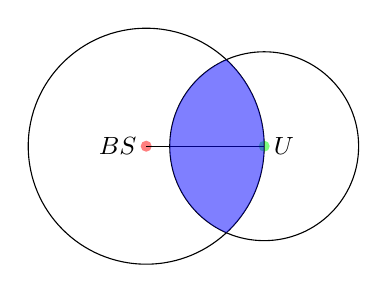
\begin{tikzpicture}[scale=0.01]
	\coordinate [label=left:{\small $BS$}] (A) at (0,0);
	\coordinate [label=right:{\small $U$}] (B) at (150,0);
	\fill [red,opacity=.5] (A) circle (200pt);
	\fill [green,opacity=.5] (B) circle (200pt);

	\draw (A) -- (B);
	\node (D) [name path=D,draw,circle through=(B)] at (A) {};
%	\node (E) [name path=E,draw,circle(60)] at (B);
	% Name the coordinates, but do not draw anything:
	\draw (B) circle(120);
	\begin{scope}
		\clip (0,0) circle(150);
		\fill[blue,opacity=.5] (150,0) circle (120);
	\end{scope}
	%	\path [name intersections={of=D and E}];

\end{tikzpicture}
\\
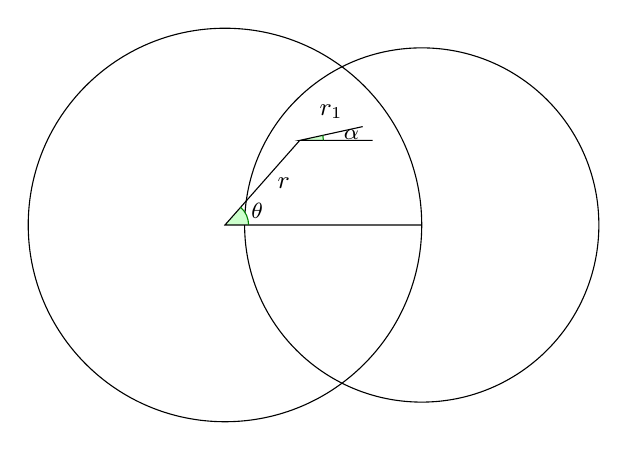
\begin{tikzpicture}[scale=0.025]
	\coordinate  (O) at (0,0);
	\coordinate  (B) at (100,0);
	\coordinate  (P) at (38,43);
	\coordinate  (U) at (75,43) ; 
	\coordinate  (Q) at (70,50);  
	\node (D) [name path=D,draw,circle through=(B)] at (O) {};
%	\node (E) [name path=E,draw,circle(60)] at (B);
	% Name the coordinates, but do not draw anything:
	\draw (B) circle(90);
	\draw (B) -- (O) -- node[right=2pt] {\small $r$} (P) pic["\footnotesize{$\theta$}",draw=green!50!black, fill=green!20, angle radius=3mm, angle eccentricity = 1.5] {angle = B--O--P};
	\draw (U) -- (P) -- node[above=2pt] {\small $r_1$} (Q) pic["\footnotesize{$\alpha$}",draw=green!50!black, fill=green!20, angle radius=3mm,angle eccentricity = 2.2] {angle = U--P--Q};
\end{tikzpicture}
\\
$
a^2 = r^2 + r_1^2 - 2r_1r\cos(180-\theta+\alpha) 
$

$
b^2 = (r\sin\theta + r_1\sin\alpha)^2 + (R_0-r\cos\theta-r_1cos\alpha)^2
$
\begin{align*}
	a^2 &> R_0^2 \Rightarrow r_1 > r_{11} \\
	b^2 &> R_2^2 \Rightarrow r_1 > r_{12}
\end{align*}
\begin{align*}
	\beta_1 &= \cos^{-1}\bigg(1-\frac{R_2^2}{2R_0^2}\bigg) - \theta \\
	\beta_2 &= \cos^{-1}\bigg(1-\frac{R_2^2}{2R_0^2}\bigg) \\
	\alpha_1 &= \theta + \tan^{-1}\bigg( \frac{R_0\sin\beta_1}{R_0\cos\beta_1-r}\bigg)\\
	\alpha_2 &= \tan^{-1}\bigg( \frac{r\sin\theta + R_0\sin\beta_2}{R_0cos\beta_2 - r\cos\theta} \bigg)
\end{align*}

\begin{equation*}
	P  = \left(
	\begin{array}{cc}
	Q & R \\
		\mathbf{0} & I_r \\
	\end{array} \right)
\end{equation*}

\begin{align*}
	N = \sum_{k=0}^{\infty} Q^k &= (I-Q)^{-1}\\
	Expected = \mathbf{t} &= N\mathbf{1} \\
	variance &= (2N-I)\mathbf{t} - \mathbf{t}_{sq}
\end{align*}

\end{document}

